\section{Examples and experiments}
\label{sec:examples}
This section describes possible examples to include in the paper.
\begin{description}
\item{\bf Visually verifiable examples:}\\
This set of examples are mostly used for validation purposes where the expected
behavior is obvious.
\begin{itemize}
    \item Rectangular bar of isotropic material with Young's modulus varying from one end
        to the other.
    \item Rectangular bar of orthotropic material with material axis rotating
        from one end to the other.
    \item A thin bar of various material properties such that, when pinching both
    ends, it deform in a zig-zag pattern instead of normal buckling. See Figure
    \ref{fig:zig_zag_bar}.
\end{itemize}
\begin{figure}
\centering
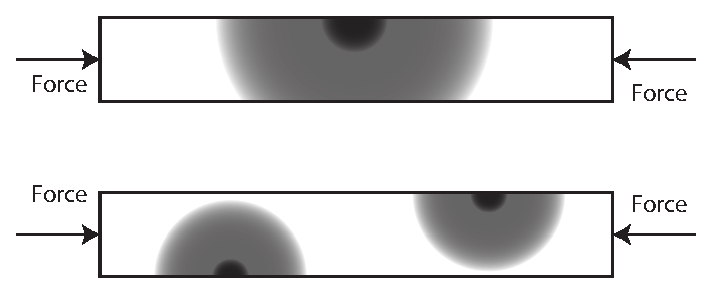
\includegraphics[width=0.5\textwidth]{images/zig_zag_bar}
\caption{White and black represent stronger and weaker material properties,
    respectively. One can achieve different bending behavior using the
material property specification above.  Top: center kink.  Bottom: Zig-zag
deformation.}
\label{fig:zig_zag_bar}
\end{figure}

\item{\bf Compare with ``Design and Fabrication of Materials with Desired
Deformation Behavior'' \cite{Bickel2010}:}\\
The goal of comparing to \cite{Bickel2010} is to show the resulting
microstructure of our approach can approximate material properties of their
layered design.  For example, we could simulate poking the slipper sole (see
their teaser) twice: once with their sole design, and once with our
microstructure pattern.  Ideally both simulations yield the same displacements
of the poking location.

\item{\bf Compare with shape/topological optimization:}\\
As pointed out in \cite{allaire2002shape} \S 4.1.2, in compliance minimization
setting, the true optimal shape configuration under a given load is given by
microstructures.  Due to the complexity of the microstructures, one often needs
to change the problem to get a quasi-optimal solution, resembling truss
networks, that can be manufactured.  Since 3D printing, especially
multi-material printers, is agnostic to complexity, we could produce shapes
with microstructure that is stronger than truss networks.

\begin{figure}
\centering
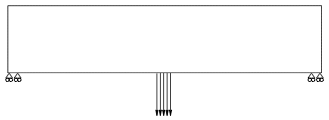
\includegraphics[width=0.5\textwidth]{images/3pt_bending}\\
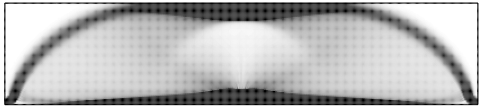
\includegraphics[width=0.5\textwidth]{images/micro_struct_bridge}\\
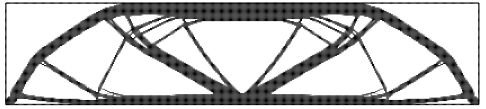
\includegraphics[width=0.5\textwidth]{images/truss_network_bridge}\\
\caption{Top: 3-point bending setup.  Middle: optimal microstructure.  The gray
region corresponds to microstructures.  Bottom:
quasi-optimal truss network.  Images taken from
\cite{allaire1996homogenization}.}
\label{fig:3pt_bending}
\end{figure}

As illustrated in Figure \ref{fig:3pt_bending}, we could print both the
microstructure bridge and the truss network bridge (note that both versions use
the same amount of material).  Subject both prints under center load and verify
the microstructure bridge is indeed stronger.  The micromaterial parameter is
part of the output of shape optimization in \cite{allaire1996homogenization}
(TODO: double check with Bob Kohn).

\item{\bf Compare with ``Computational Design of Actuated Deformable
Characters''
\cite{Skouras:2013}:}\\
One of the more practical applications is to print toy characters that can be
deformed into target poses.  In contrast to \cite{Skouras:2013}, our approach
can achieve the same effect with a single material.
(TODO: how to generate desired material tensors.)

\item{\bf Weight differentiator:}\\
This example aims to motivate real-life applications of our work.  With
microstructure, one can achieve some cool nonlinear deformation effects. Figure
\ref{fig:weight_differentiator} illustrates the desired material properties for
building a simple ``weight differentiator.''  In particular, when the device is
subject to a small load, the top surface tilts leftward.  When the load is large,
the top surface tilts rightward.  This allows one to partition balls by weight
(e.g. drop a ball on it, and the ball will bounce to the either left or right
depending on its weight).

\begin{figure}
\centering
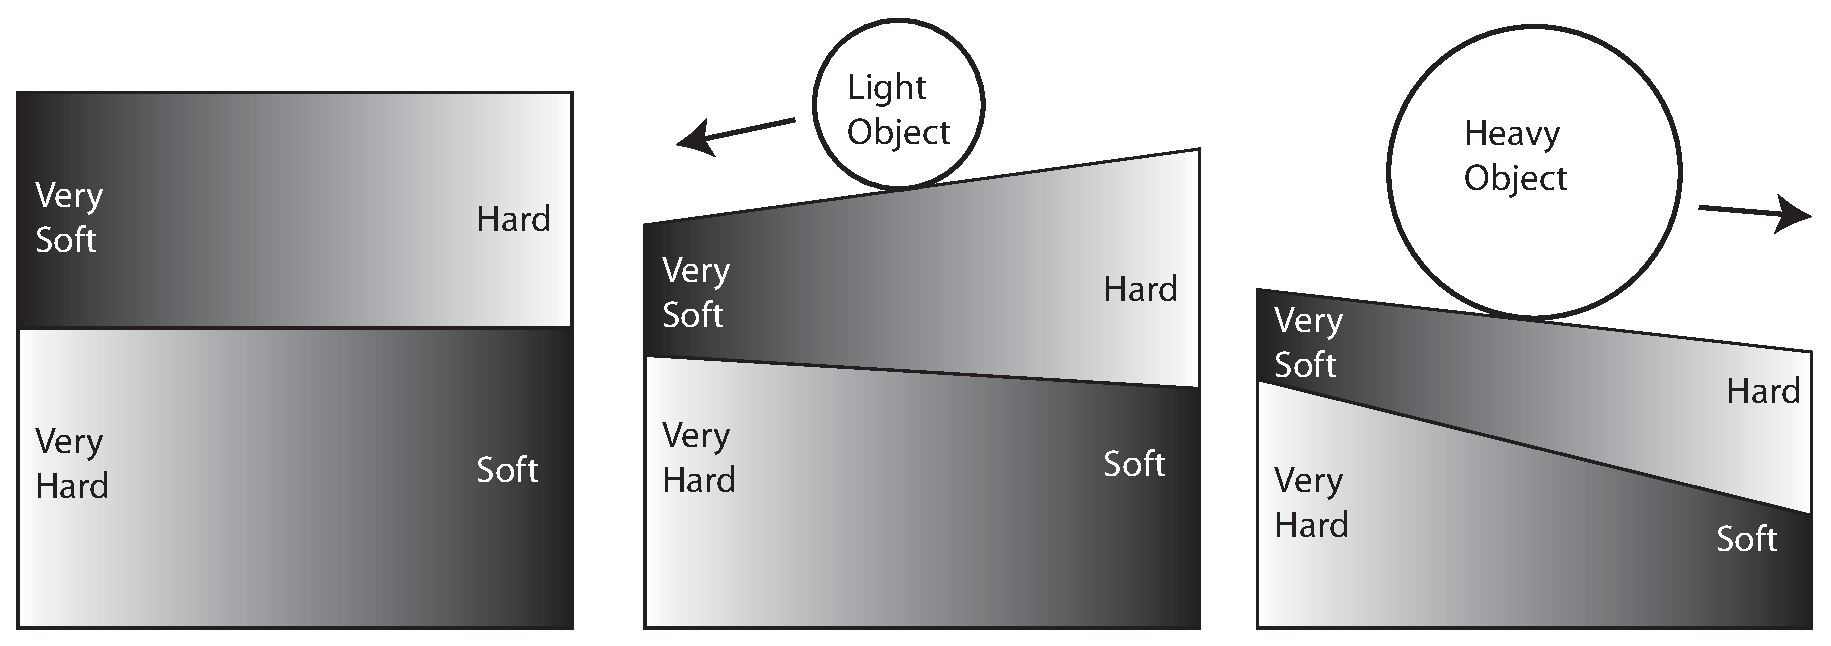
\includegraphics[width=0.9\textwidth]{images/weight_differentiator}
\caption{
The weight differentiator is a purely static mechanical device to distinguish balls
with weight above or below a certain threshold.
Left: material specification of a cube.  Middle: under light
compressive force, the top surface tilts leftward.  Right: under heavy
compressive force, the top surface tilts rightward.}
\label{fig:weight_differentiator}
\end{figure}

\end{description}

Besides the examples above, we would need to carry out physical experiments to
validate the material properties of microstructures.  Here are the proposed
experiments:

\begin{description}
\item{\bf Determine the base material's properties:}\\
We need to determine the material properties of our base material to do any
physical validation.

\item{\bf Validate sequential lamination formula in the fabrication setting:}\\
Specifically, validate equation 2.64 (p. 127) for multi-material rank-1 laminates, 2.67 for
rank-2 and 3 laminates, and 2.151 (p. 167) for single-material laminates in
\cite{allaire2002shape}.  The experiment would be 3-point bending test of
perfectly tiled microstructures. For microstructures of various length scales, we
apply a load at its center and record the corresponding displacements.  Under
infinite microstructure refinement, the extrapolated displacement should match
the displacement simulated using the formula's output elasticity tensor.

\item{\bf Validate the synthesis algorithm (Section \ref{sec:gen_connect}):}\\
For most shapes, we won't be able to tile our pattern perfectly.  Thus an
experiment validation would be necessary to test whichever algorithm we choose to
generate the microstructures.  Again, the 3 point bending test described above could
be used.  In this case, the samples should contain a microstructure that cannot
be perfectly tiled (e.g. the bar in Figure \ref{fig:zig_zag_bar}). We should
also try an object with a less trivial geometry, like a bar with large notches.

\end{description}

